\documentclass[a4paper,12pt]{article}

%%% Работа с русским языком
\usepackage{cmap}					% поиск в PDF
\usepackage{mathtext} 				% русские буквы в формулах
\usepackage[T2A]{fontenc}			% кодировка
\usepackage[utf8]{inputenc}			% кодировка исходного текста
\usepackage[english,russian]{babel}	% локализация и переносы
\usepackage{xcolor}
\usepackage{hyperref}
 % Цвета для гиперссылок
\definecolor{linkcolor}{HTML}{799B03} % цвет ссылок
\definecolor{urlcolor}{HTML}{799B03} % цвет гиперссылок

\hypersetup{pdfstartview=FitH,  linkcolor=linkcolor,urlcolor=urlcolor, colorlinks=true}

%%% Дополнительная работа с математикой
\usepackage{amsfonts,amssymb,amsthm,mathtools} % AMS
\usepackage{amsmath}
\usepackage{icomma} % "Умная" запятая: $0,2$ --- число, $0, 2$ --- перечисление

%% Номера формул
%\mathtoolsset{showonlyrefs=true} % Показывать номера только у тех формул, на которые есть \eqref{} в тексте.

%% Шрифты
\usepackage{euscript}	 % Шрифт Евклид
\usepackage{mathrsfs} % Красивый матшрифт

%% Свои команды
\DeclareMathOperator{\sgn}{\mathop{sgn}}

%% Перенос знаков в формулах (по Львовскому)
\newcommand*{\hm}[1]{#1\nobreak\discretionary{}
{\hbox{$\mathsurround=0pt #1$}}{}}
% графика
\usepackage{graphicx}
\graphicspath{{pictures/}}

\usepackage[left=25mm, top=30mm, right=25mm, bottom=30mm, nohead, nofoot]{geometry}


\DeclareGraphicsExtensions{.pdf,.png,.jpg}
\author{Бурмашев Григорий, БПМИ-208}
\title{Язык SQL,  дз -- 9  }
\date{\today}
\begin{document}
\maketitle
\section*{Номер 3}
\begin{center}
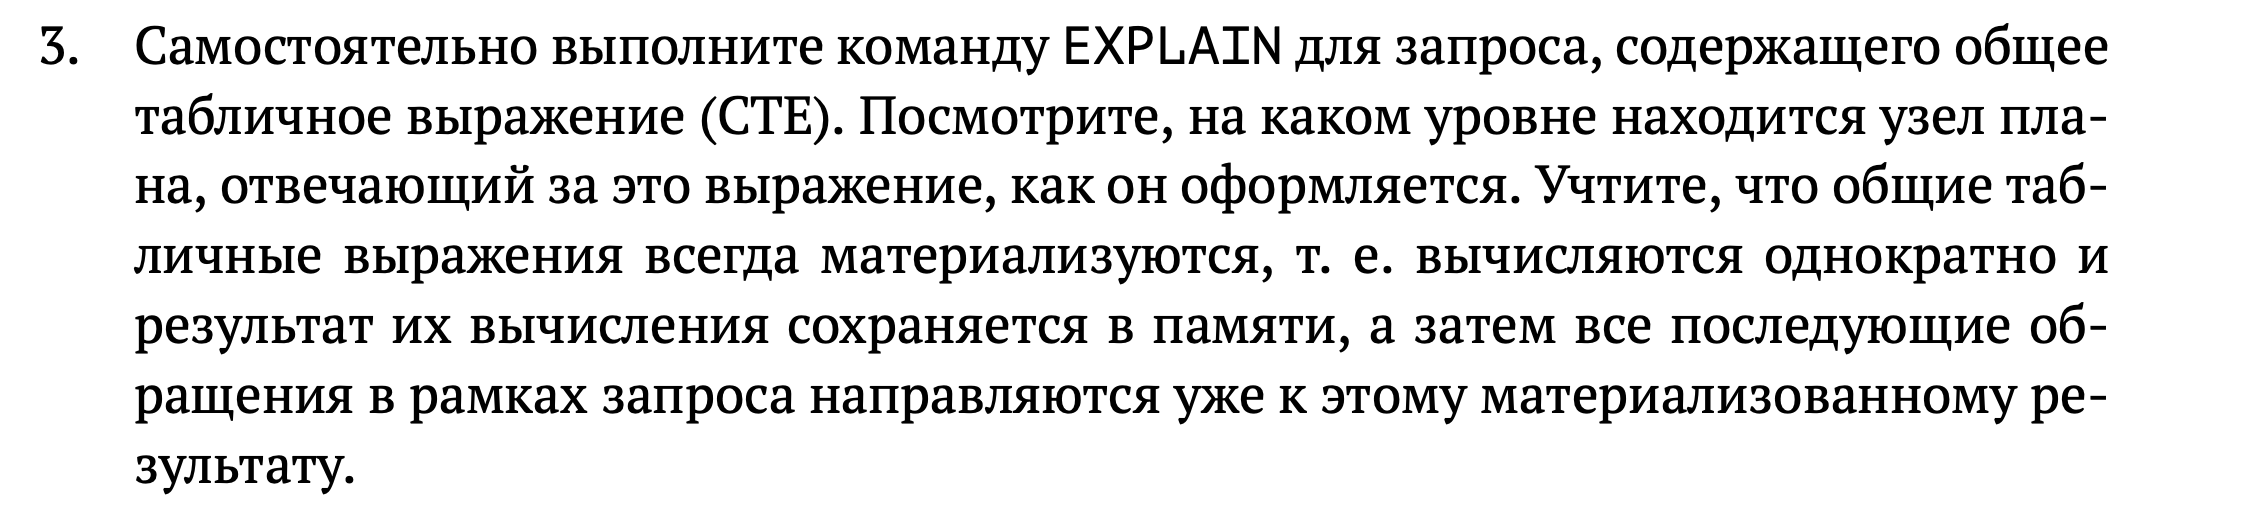
\includegraphics[scale=0.4]{t3.png}
\end{center}
Посмотрим на запрос из одной из предыдущих домашних заданий, который содержит в себе CTE:
\begin{center}
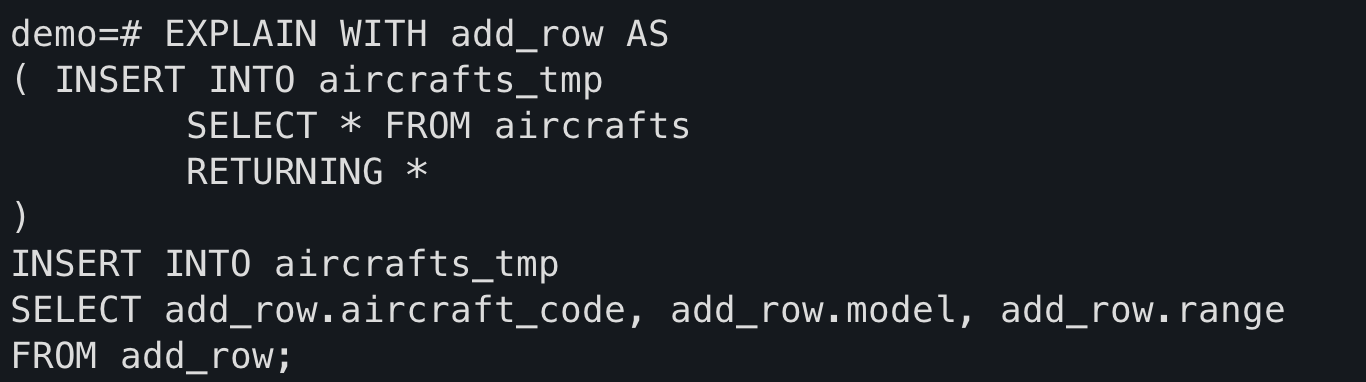
\includegraphics[scale=0.6]{31.png}
\end{center}
Результат:
\begin{center}
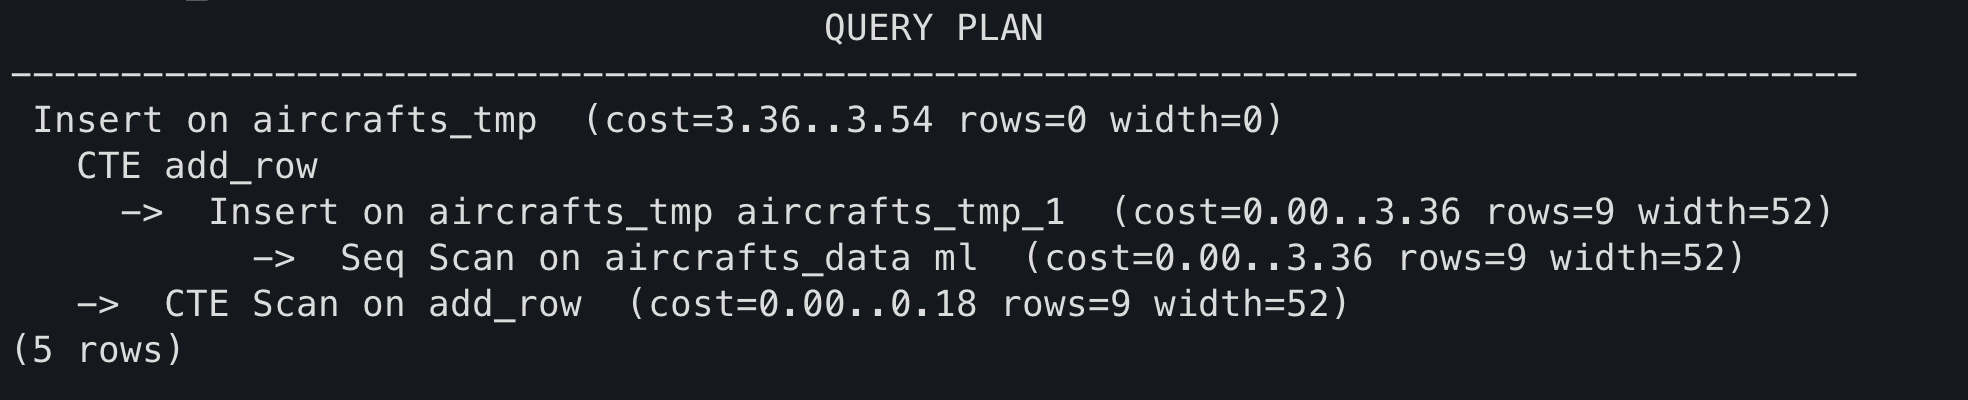
\includegraphics[scale=0.5]{32.png}
\end{center}
Узел CTE находится на самом верху в плане, я ожидал, что он будет самым внутренним (приоритетным), поскольку CTE мы (кажется) должны создать в первую очередь.
\clearpage
\section*{Номер 6}
\begin{center}
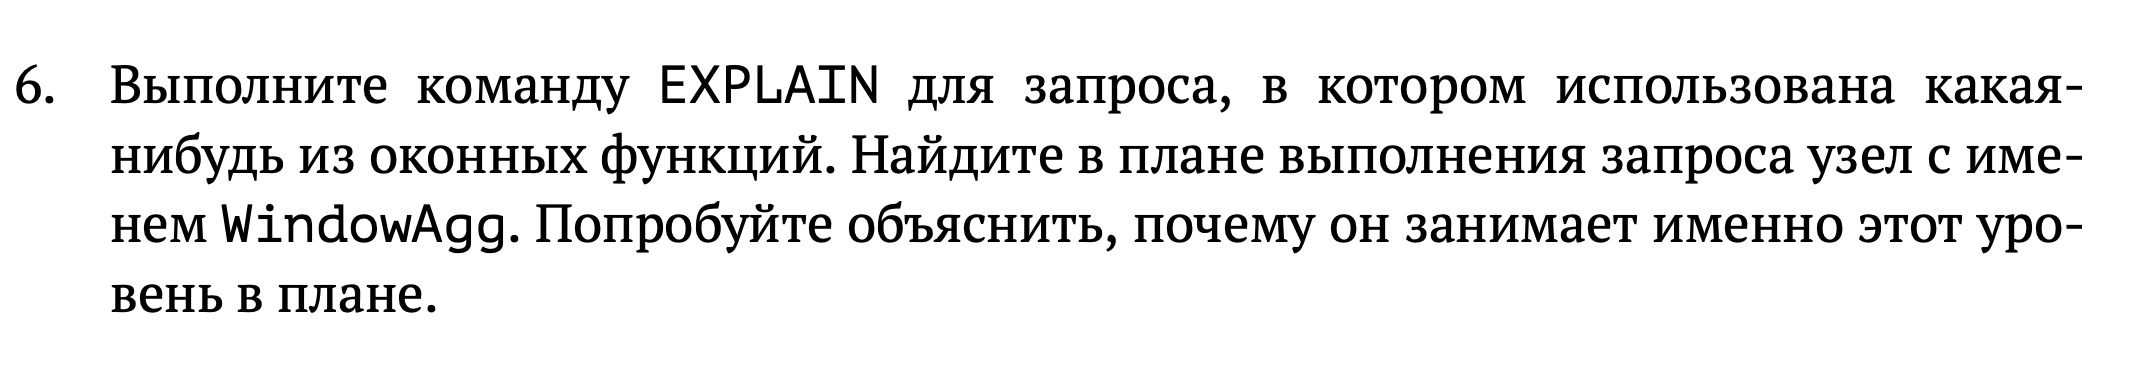
\includegraphics[scale=0.4]{t6.png}
\end{center}
Делаю команду и сразу смотрю на результат:
\begin{center}
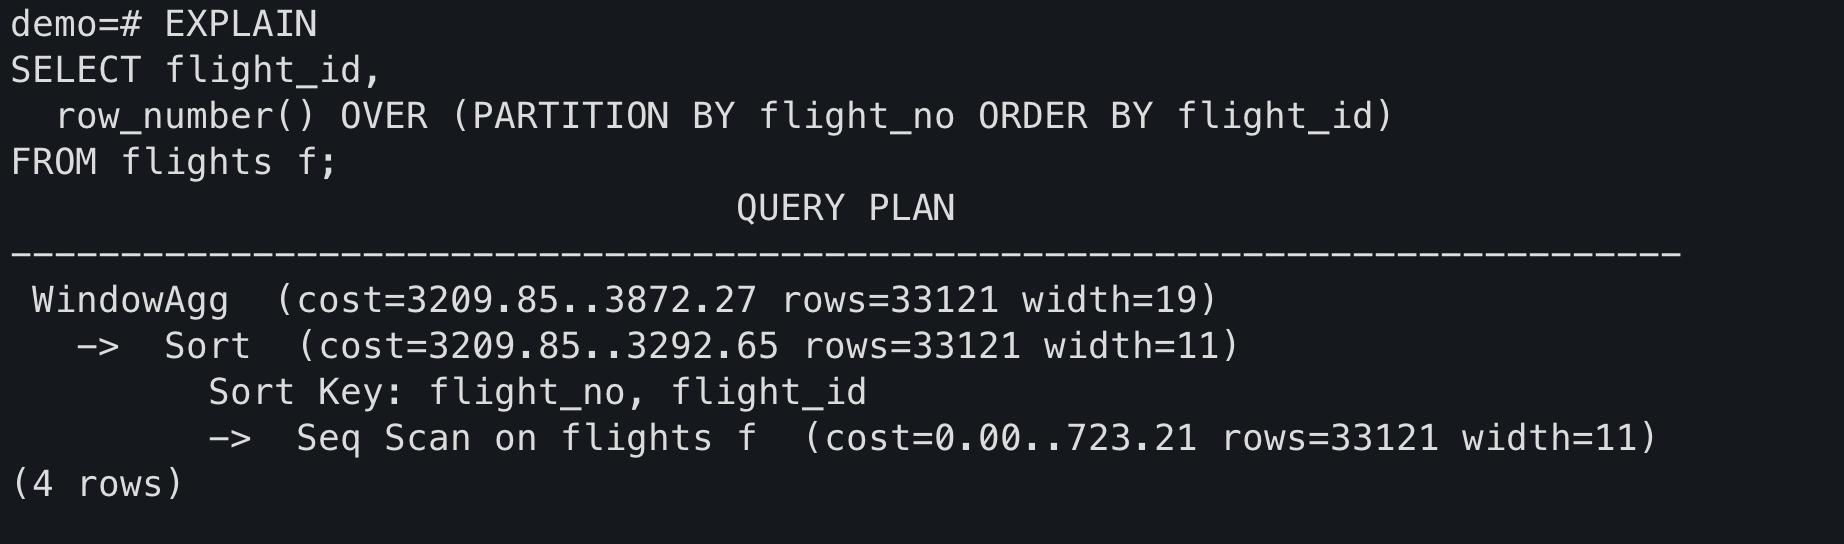
\includegraphics[scale=0.6]{63.png}
\end{center}
Здесь WindowAdd идет самым первым, поскольку он вычисляет оконную функцию по тому (OVER) набору данных, который был отсортирован с помощью ORDER BY (Sort ...)
\clearpage
\section*{Номер 8}
\begin{center}
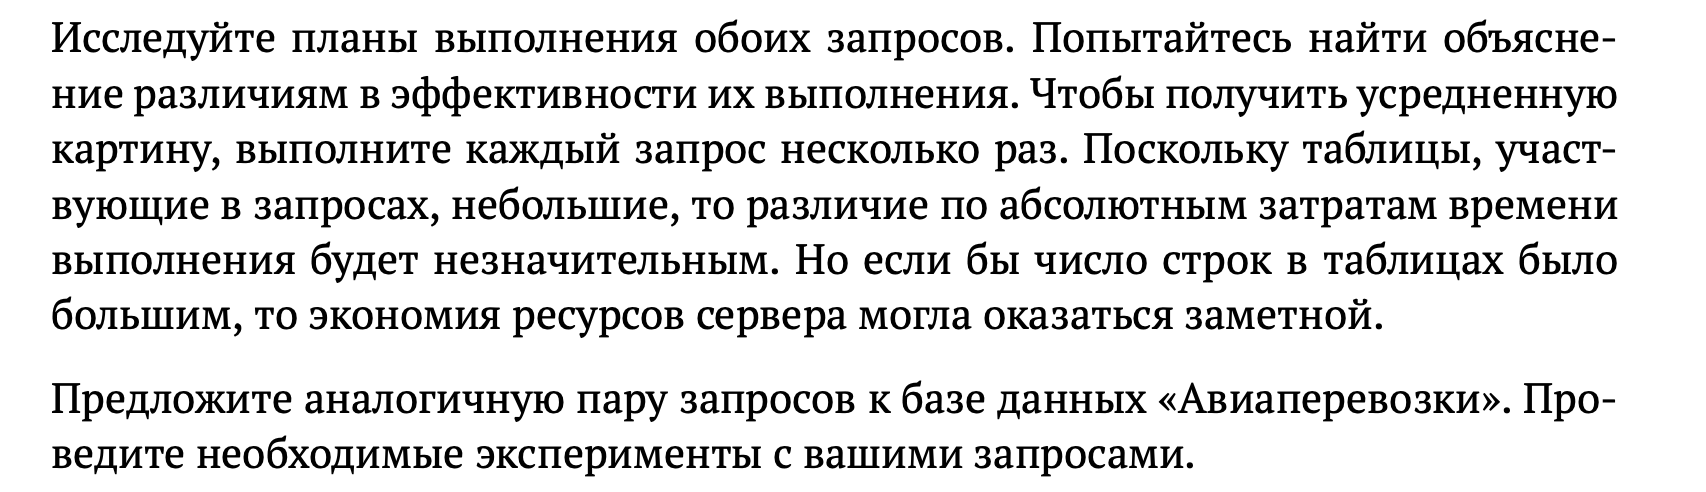
\includegraphics[scale=0.4]{t8.png}
\end{center}
Проверяю время выполнения первого запроса:
\begin{center}
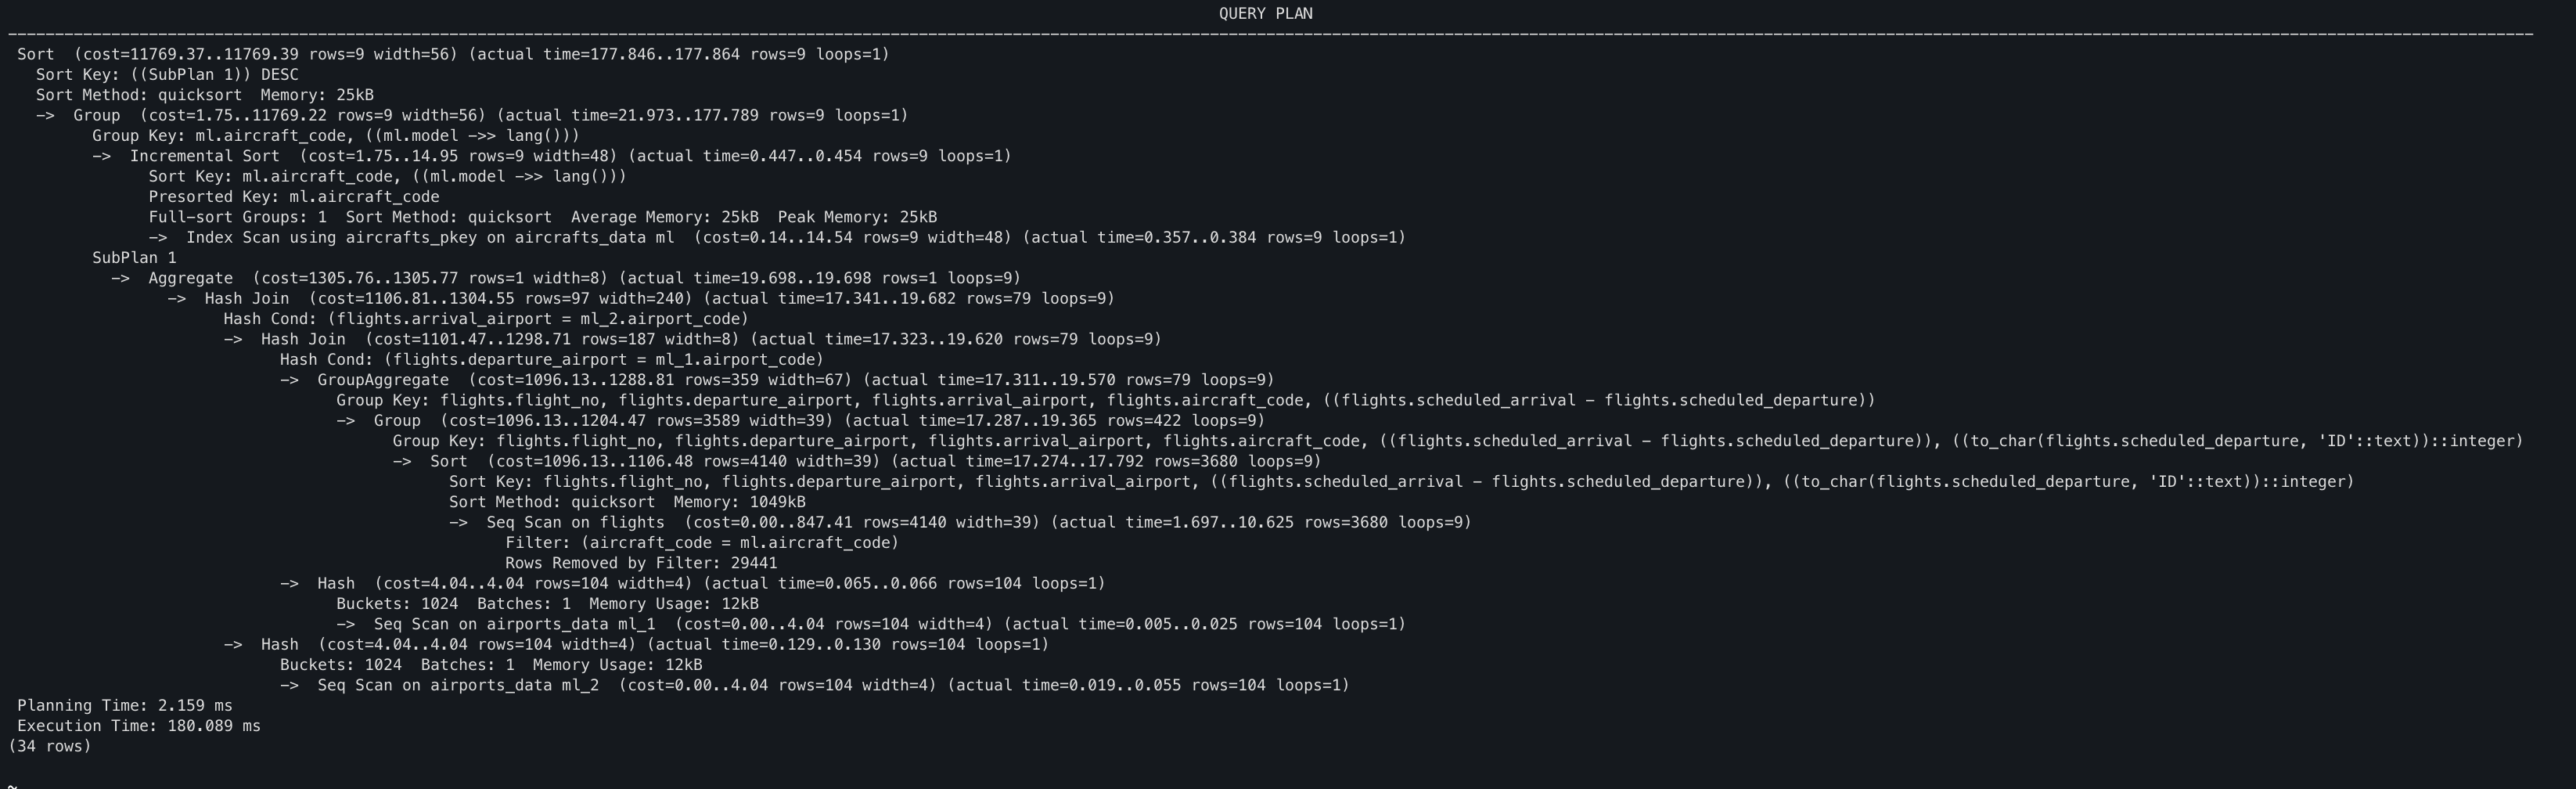
\includegraphics[scale=0.4]{81.png}
\end{center}
Делаю еще пару запусков:
\begin{center}
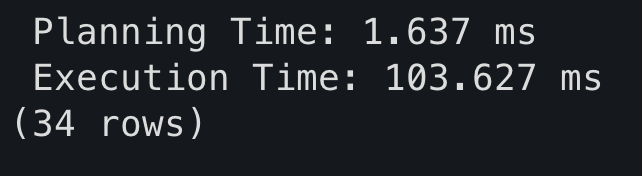
\includegraphics[scale=0.6]{82.png}
\end{center}
\begin{center}
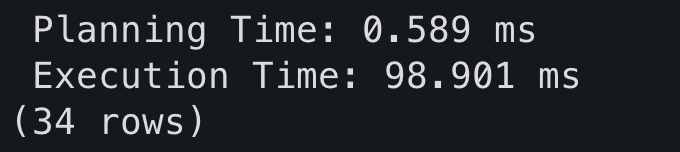
\includegraphics[scale=0.6]{83.png}
\end{center}
Второй запрос:
\begin{center}
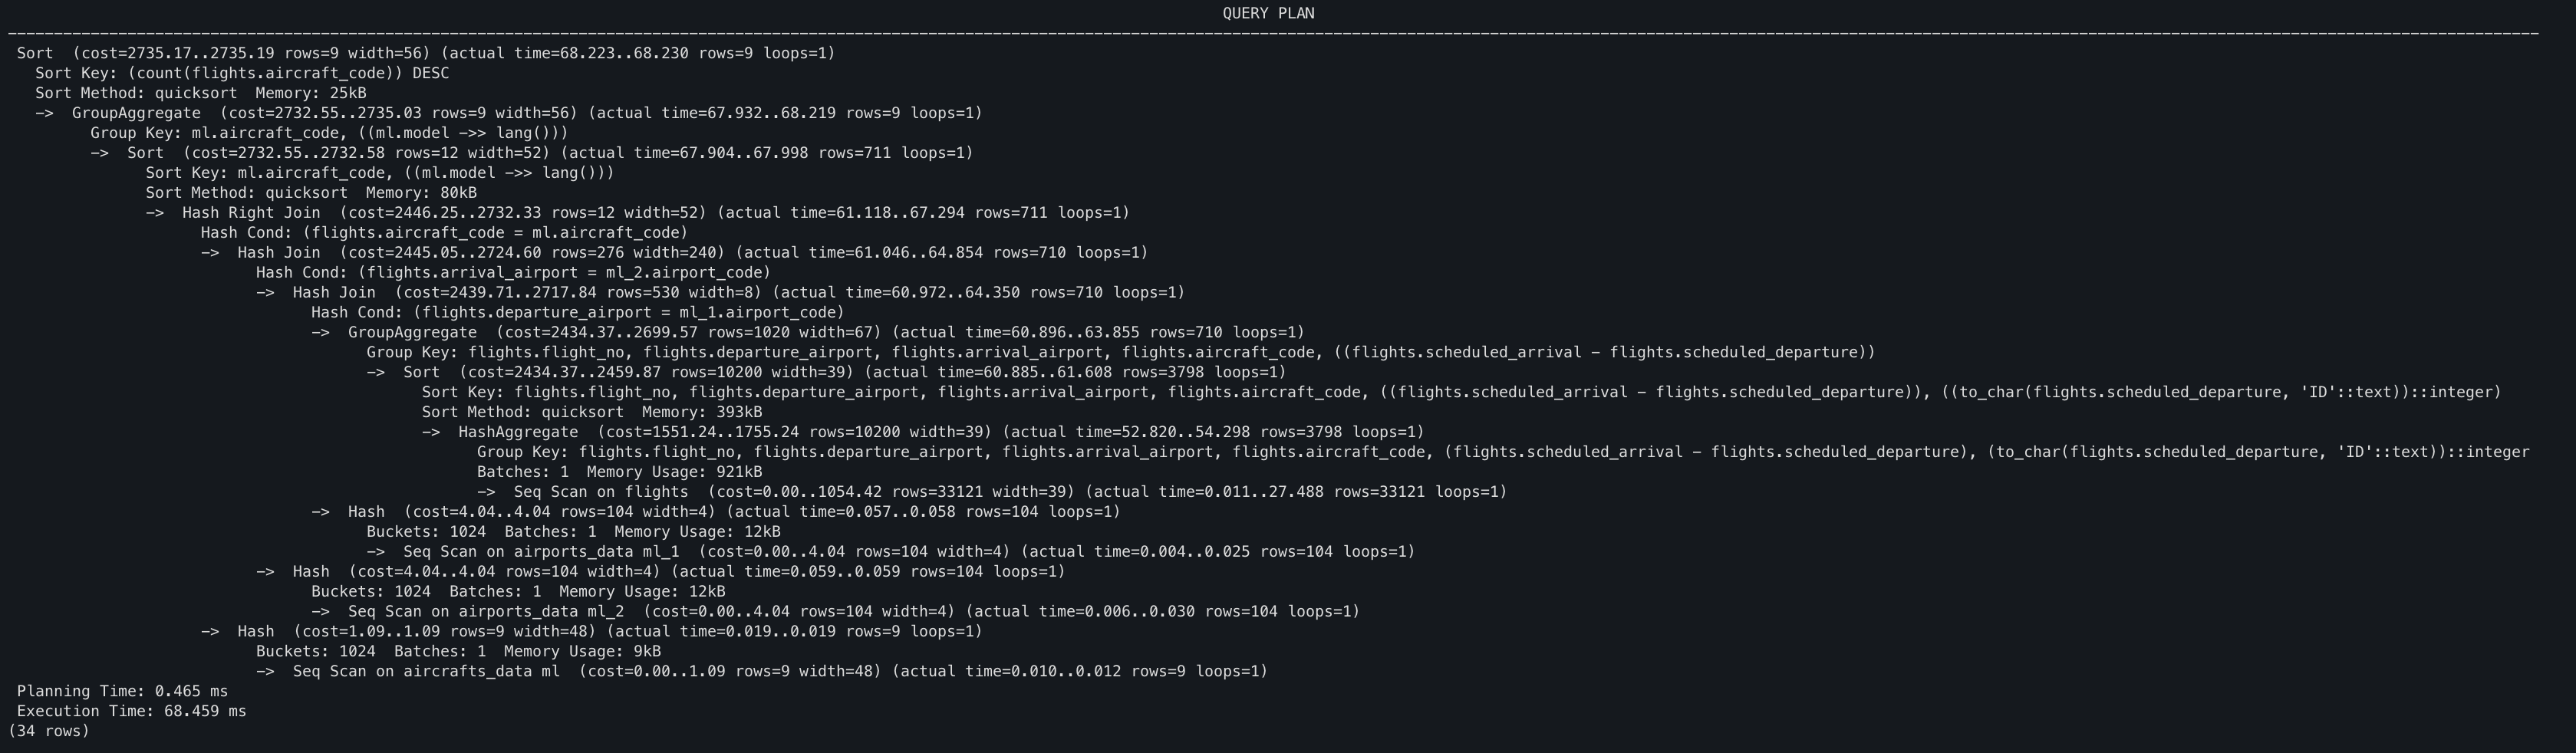
\includegraphics[scale=0.3]{84.png}
\end{center}
\begin{center}
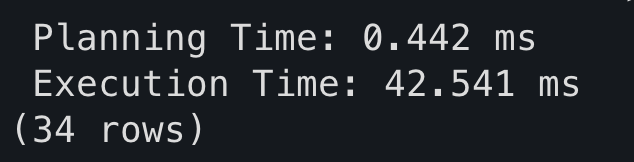
\includegraphics[scale=0.6]{85.png}
\end{center}
\begin{center}
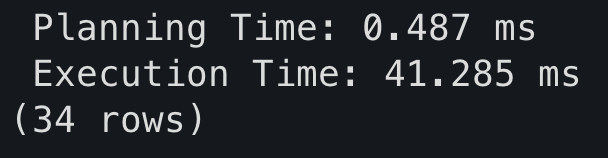
\includegraphics[scale=0.6]{86.png}
\end{center}
Видим, что для обоих запросов planning time \textbf{очень} сильно отличается (в меньшую сторону) от execution time. Planning time не учитывает в себе то время, что сервер в реальности затратит на обработку запроса и выдачу результата. При этом для второго запроса оба времени меньше, что ожидаемо, поскольку мы оптимизировали запрос путем замены коррелированного запроса на JOIN. 
\\\\
Теперь придумаем аналогичные запросы. Первый:
\begin{center}
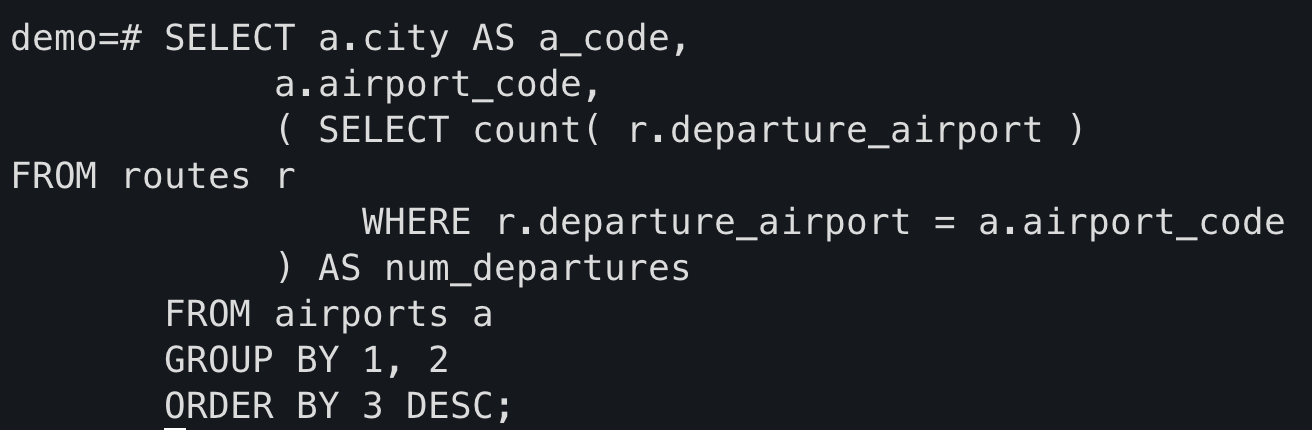
\includegraphics[scale=0.6]{87.png}
\end{center}
Время выполнения:
\begin{center}
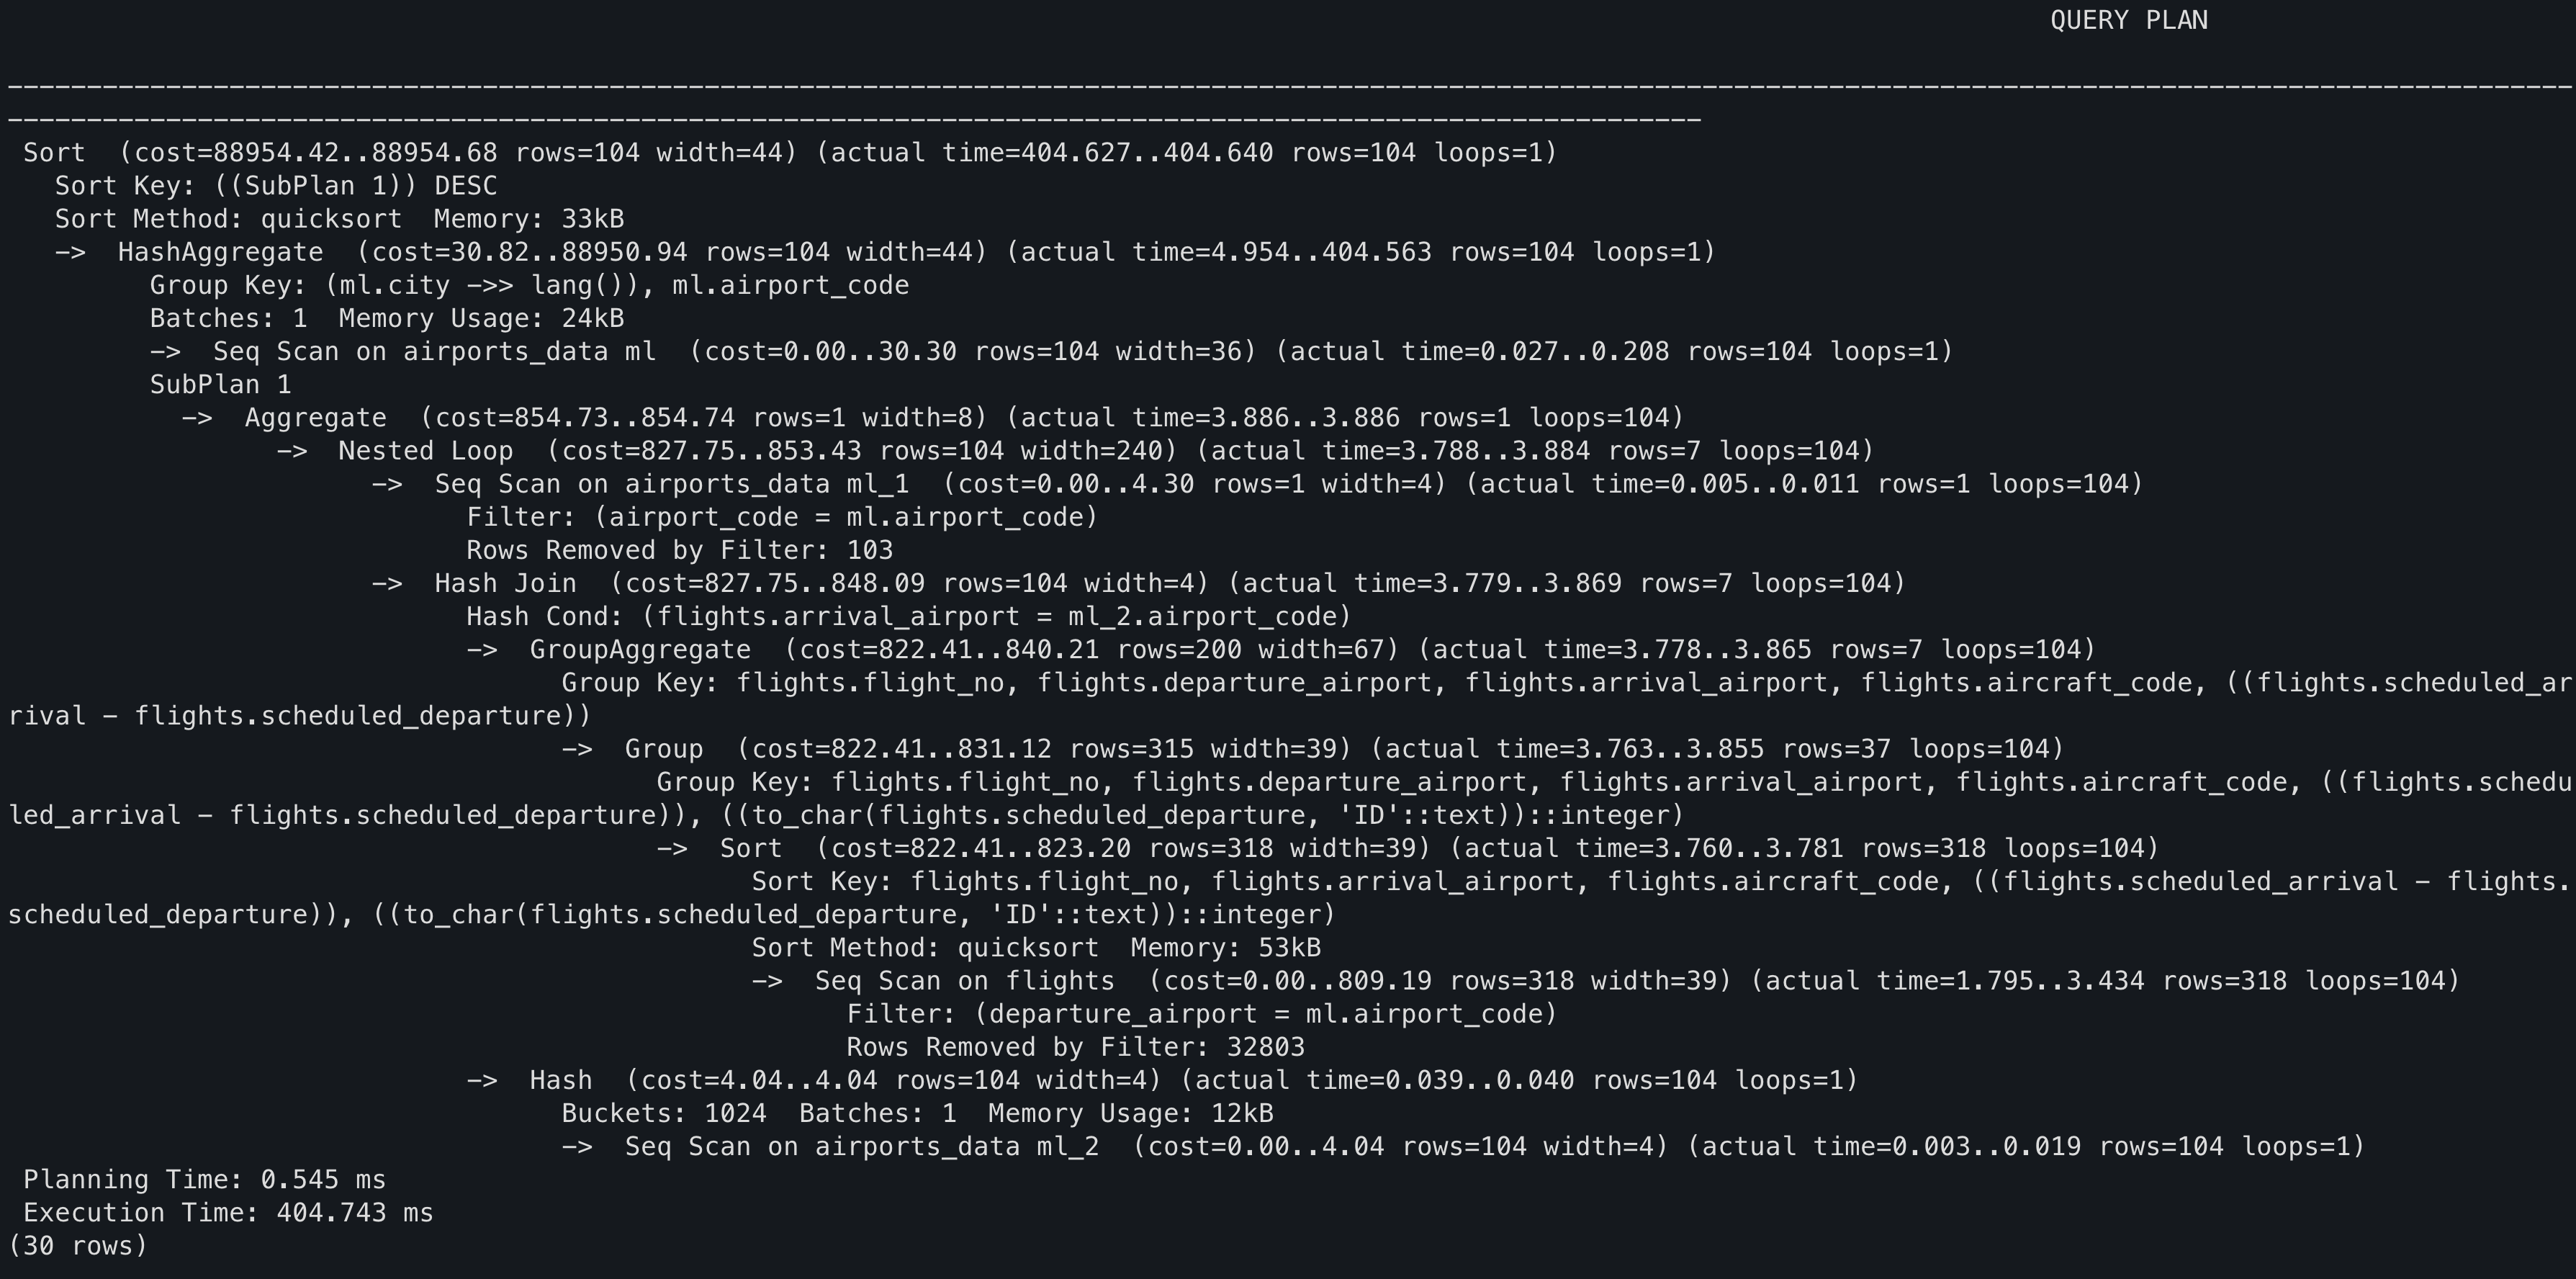
\includegraphics[scale=0.3]{88.png}
\end{center}
\begin{center}
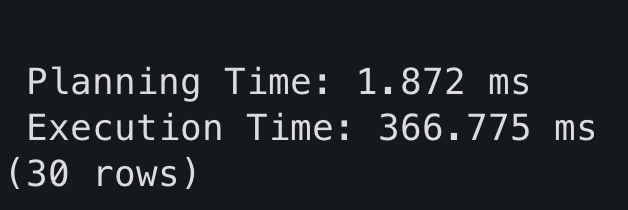
\includegraphics[scale=0.6]{89.png}
\end{center}
Второй запрос:
\begin{center}
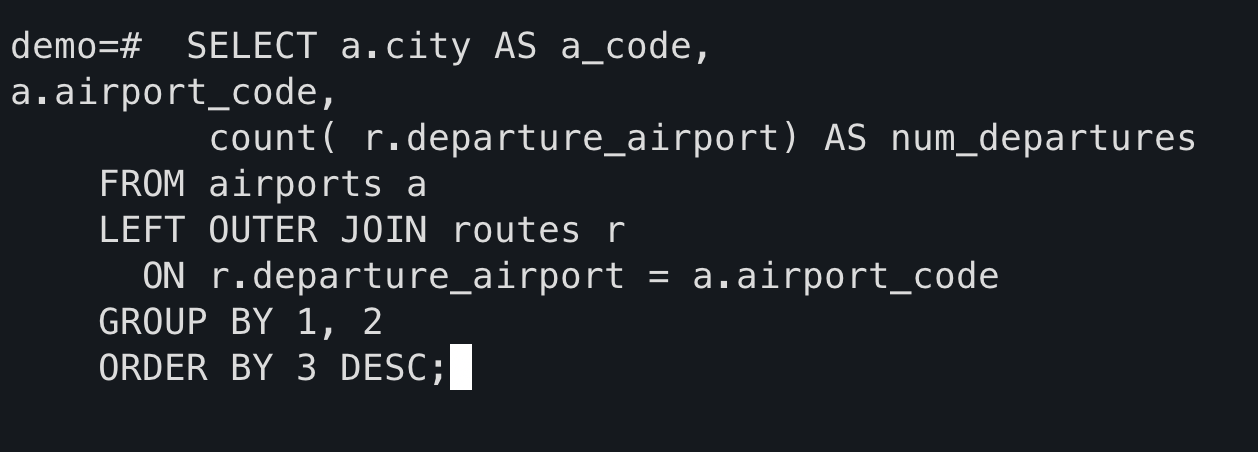
\includegraphics[scale=0.6]{810.png}
\end{center}
Время выполнения:
\begin{center}
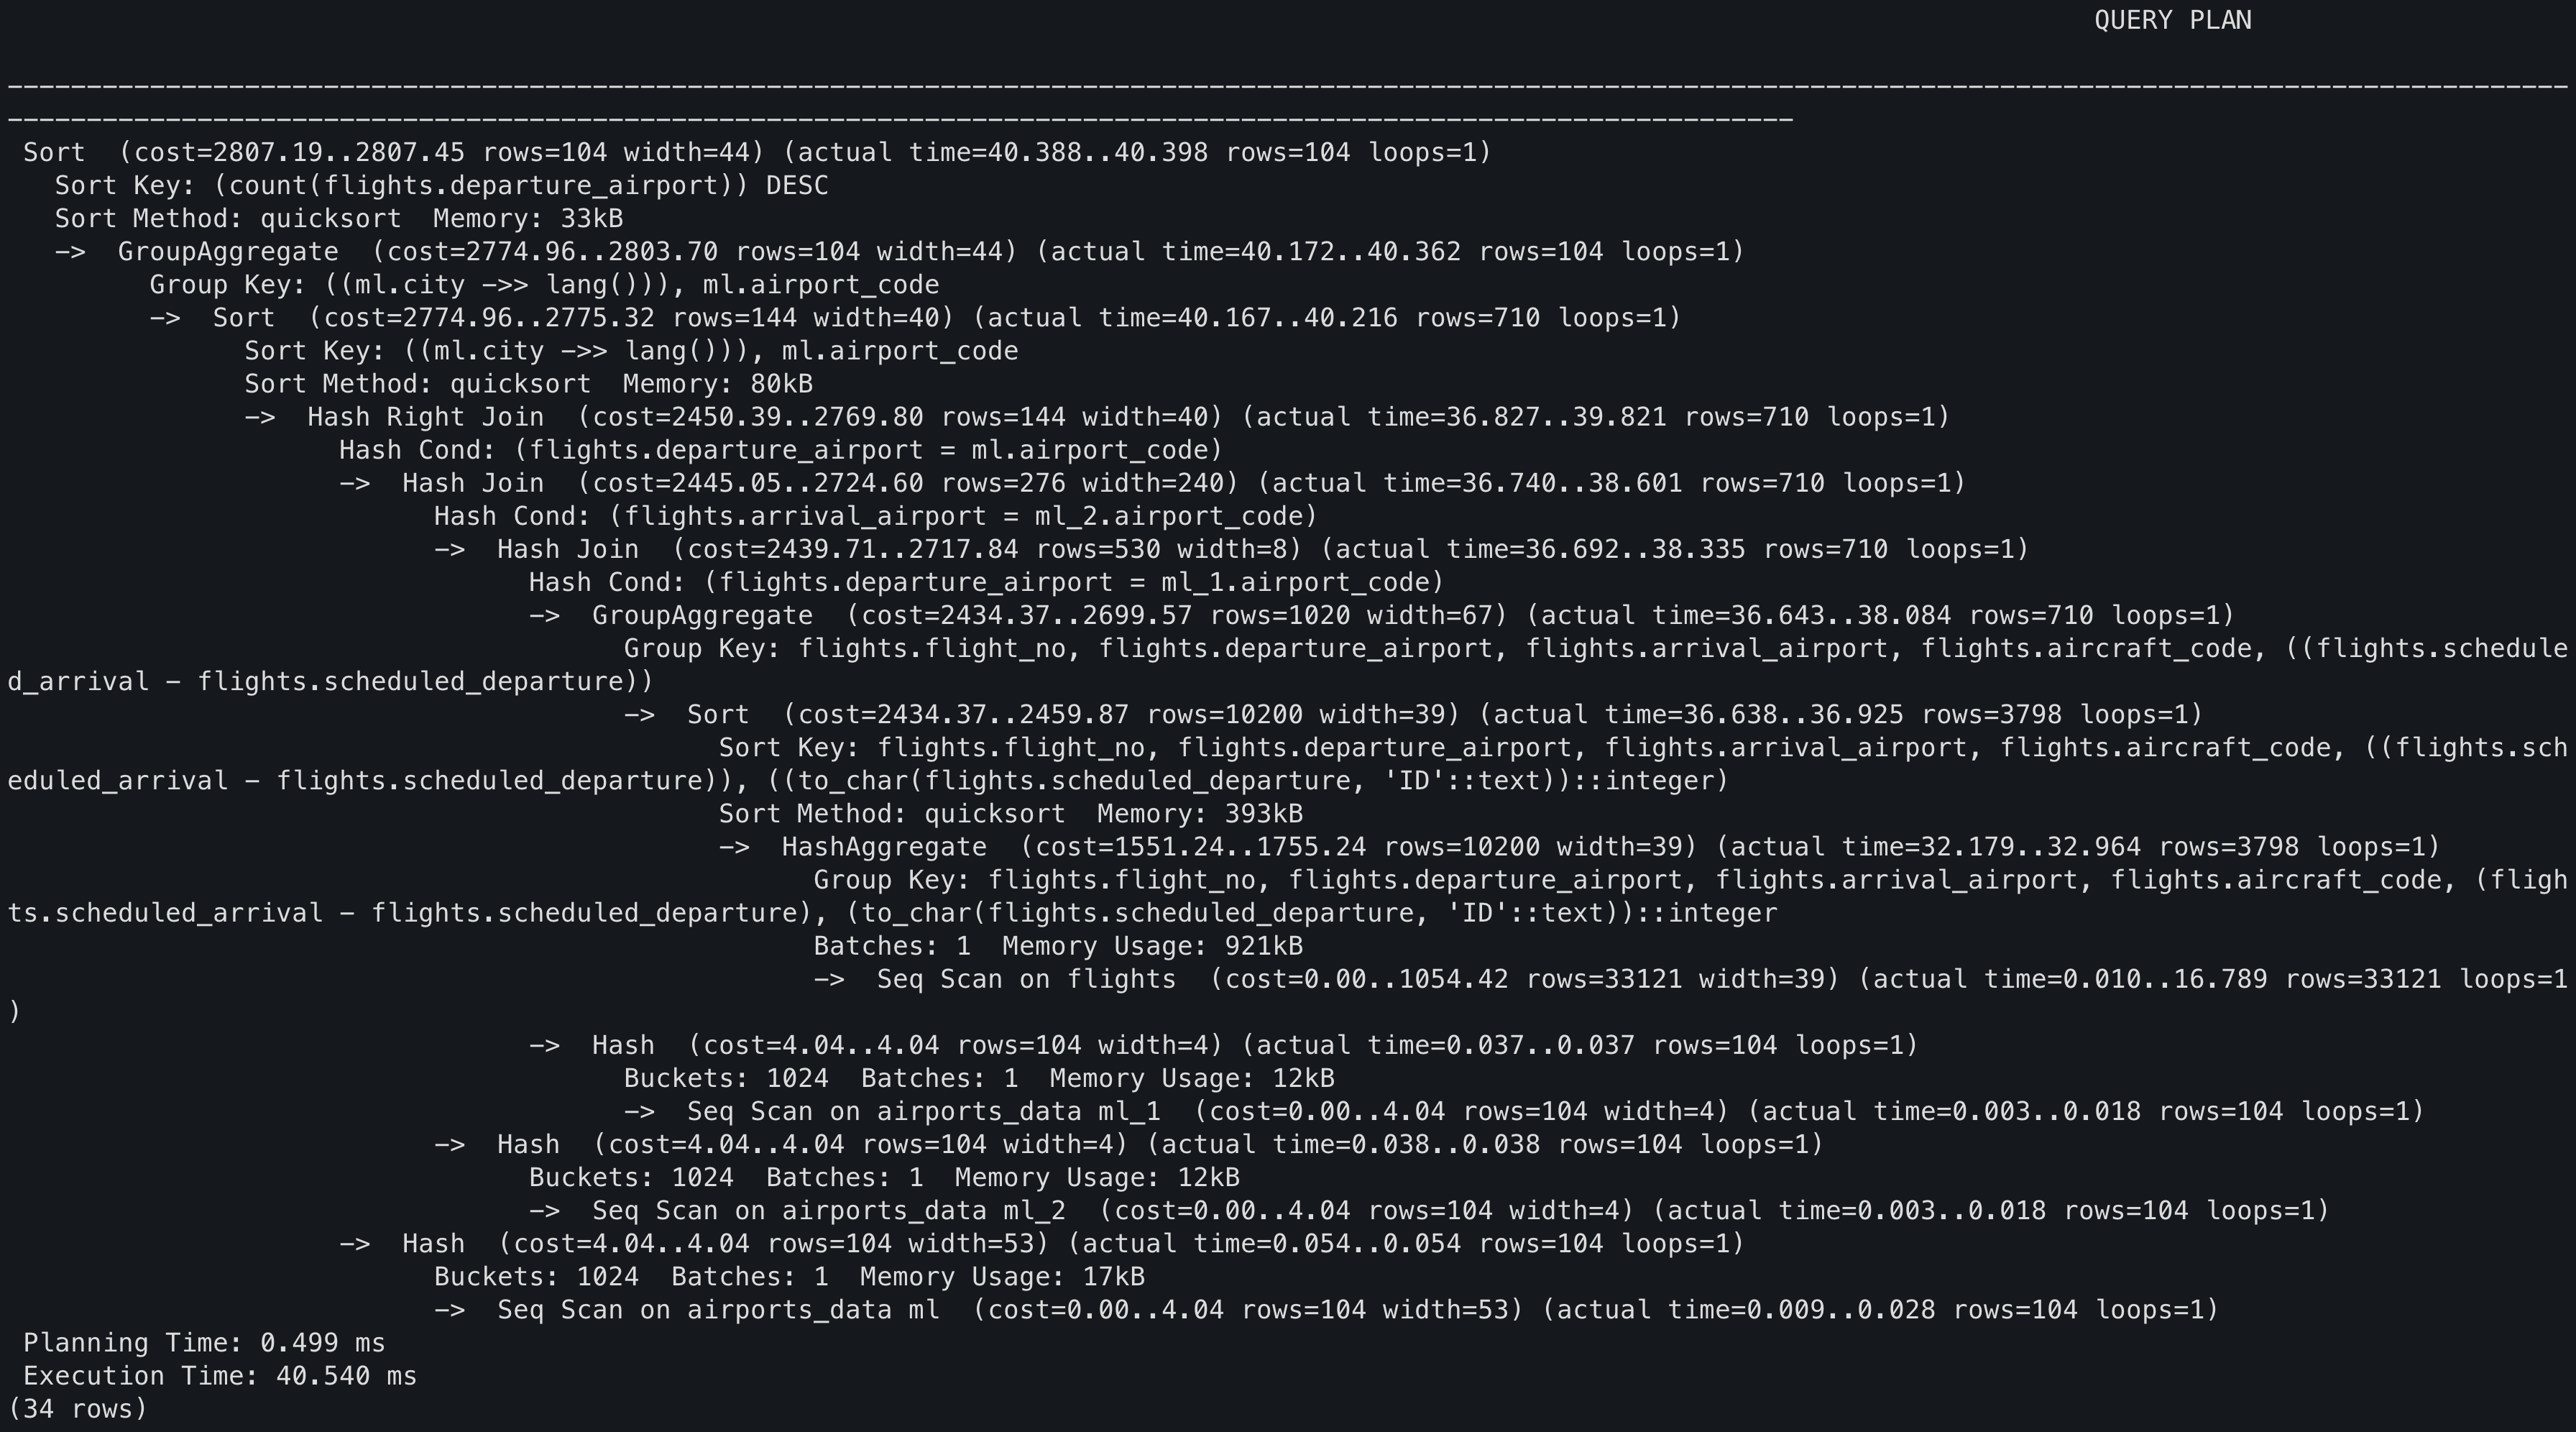
\includegraphics[scale=0.3]{811.png}
\end{center}
\begin{center}
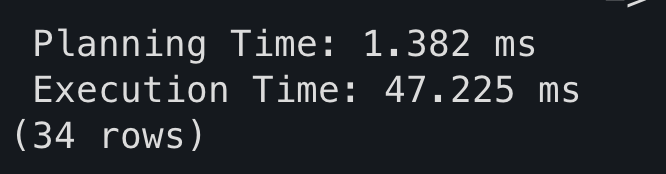
\includegraphics[scale=0.6]{812.png}
\end{center}
\begin{center}
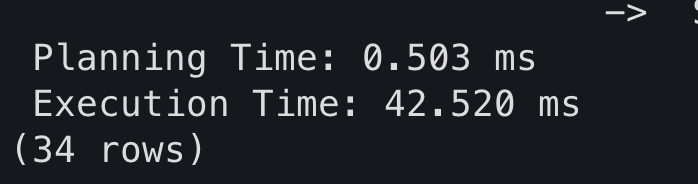
\includegraphics[scale=0.6]{813.png}
\end{center}
Получили аналогичный результат, время выполнения ведет себя точно также при оптимизации.
\end{document}
